
\section{Results}          
\subsection{Experimental Set up}    
In order to test the performance of the system an existing twitter corpus, provided by Sanders Analytics, was used. This data is for training and testing analysis algorithms. It consists of 5513 hand-classified tweets. Each tweet was classified with respect to one of four different topics (microsoft, twitter, apple, google). The format for this corpus it is described in table \ref{table:dataformat}:
\begin{table}[ht]
\centering
    \begin{tabular}{  l  l }
    \toprule
	Field & Content \\
	\midrule    
	 Query & apple	\\
	 Sentiment &	positive \\
	 TweetID & 126322063332999169 \\
	 Date	& Tue Oct 18 15:41:41 +0000 2011 \\
	 Content & apple is efffing amazing!! \\
	\bottomrule
      \end{tabular}
\caption{Format of Data}      
     \label{table:dataformat}
\end{table}

Part of this corpus was used to train the Bayes classifier, and part of it was used to test the performance of all the implemented algorithms. Prior to the testing and training we used some preprocessing techniques to achieve better results. These are annotations and URL' s removal and  elimination of repeated letters. In addition to this, a list of smilies has been added to the lexicon because they can express positive and negative emotions.

The annotations like \emph{@someone} and URL's have been removed because they add significant noise to the sentiment analysis. For the same reason we mapped the repeated letters like in the word greeaaaaaat to just a double occurrence of them. e.g greeaaaaat is transformed to greeaat. This mapping is used in order to avoid adding additional noise, if by mistake correct repeated letters are eliminated. e.g look to lok.

The metrics which have been used to measure the effectiveness of our system are \emph{precision} and \emph{recall}.
Precision is the fraction of correctly classified documents, while recall is the fraction of non-neutral tweets. The formulas that indicate these fractions are the following.
\begin{equation}
precision = \frac{TruePositive}{TruePositive + FalsePositive }
\end{equation}
\begin{equation}
recall = \frac{TruePositive}{TruePositive + FalseNegative}
\end{equation}
By the terms \emph{positive} and \emph{negative} we mean the positive and negative sentiments. In our case we are mainly interested in controlling the fraction of true Positives and true Negatives tweets returned by our algorithm rather than taking into account the fraction of  the neutral tweets in comparison with the positive and negatives. Thus, we measured the fraction of the correct positive/negative and false positive/negative classifications.

Finally, we used tweets which are written only in English and the testing query was "Microsoft". 


\subsection{Results}
Four different methods have been used for sentiment estimation. The Gaussian distance, the detection of negations and modifiers, the bayes classifier and a lexicon with assigned negative and positive scores. In addition to this we measured the impact of the presence of smilies on the sentiment score. Figure \ref{unfiltereddata} illustrates the performance of the algorithms described above for unfiltered data, which means without annotations / URL removal, and without the elimination of repeated characters. From the figure it is clear that smilies have a very strong impact on the sentiment analysis, as they have perfect precision and recall. The Bayes classifier appears to have a low precision score because of the high dimensionality of the data. However, it gives a very good score for recall.
\begin{figure}[ht]
\centering
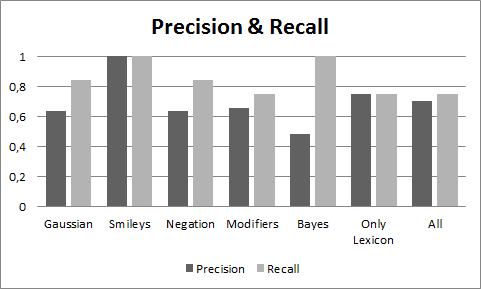
\includegraphics[width=0.5\textwidth]{images/unfiltereddata.png}
\label{unfiltereddata}
\caption{Precision and Recall for unfiltered data.}
\end{figure}

After the preprocessing step, the algorithm's performance has been measured again and the results are shown in figure \ref{nonannotateddata} and figure \ref{nonmultiplesdata}. The recall is affected by the filtering, the noise has been eliminated from the data and a significant improvement occurs at recall for the negations and the modifiers. However, the performance of precision has decreased. The Bayes classifier does not indicate any difference.  Finally, the overall score has an improvement too in comparison with the unfiltered data.  
\begin{figure}[ht]
\centering
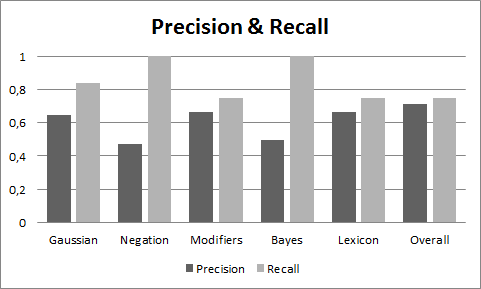
\includegraphics[width=0.5\textwidth]{images/nonannotadeddata.png}
\label{nonannotateddata}
\caption{Precision and Recall for data without URL's and annotation.}
\end{figure}

\begin{figure}[ht]
\centering
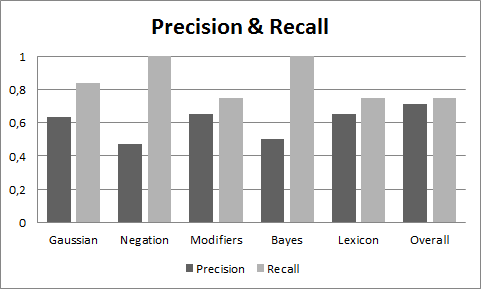
\includegraphics[width=0.5\textwidth]{images/eliminatedmultiplesdata.png}
\label{nonmultiplesdata}
\caption{Precision and Recall for data without repeated characters.}
\end{figure}

The overall performance of the algorithm is near 0.71 for precision and 0.75 for recall.